\documentclass{article}

\usepackage{arxiv}

\usepackage[utf8]{inputenc} % allow utf-8 input
\usepackage[T1]{fontenc}    % use 8-bit T1 fonts
\usepackage{hyperref}       % hyperlinks
\usepackage{url}            % simple URL typesetting
\usepackage{booktabs}       % professional-quality tables
\usepackage{amsfonts}       % blackboard math symbols
\usepackage{nicefrac}       % compact symbols for 1/2, etc.
\usepackage{microtype}      % microtypography
\usepackage{lipsum}		% Can be removed after putting your text content
\usepackage{amssymb,amsmath,amsthm}
\usepackage{listings}
\usepackage{graphicx}
\usepackage{subfig}
\usepackage{apacite}
\usepackage{algorithm}
\usepackage{algorithmicx}
\usepackage{algpseudocode}
\usepackage{kbordermatrix}% http://www.hss.caltech.edu/~kcb/TeX/kbordermatrix.sty
\usepackage{todonotes}

\newtheorem{theorem}{Theorem}
\DeclareMathOperator\supp{supp}

\title{Data assimilation with agent-based models: A sampling algorithm}

%\date{September 9, 1985}	% Here you can change the date presented in the paper title
%\date{} 					% Or removing it

\author{
  Daniel Tang\\
    Leeds Institute for Data Analytics, University of Leeds, UK\thanks{This project has received funding from the European Research Council (ERC) under the European Union’s Horizon 2020 research and innovation programme (grant agreement No. 757455)}\\
  \texttt{D.Tang@leeds.ac.uk}\\
  \AND
  Nick Malleson\\
  School of Geography, University of Leeds, UK\\  
  %% examples of more authors
  %% \AND
  %% Coauthor \\
  %% Affiliation \\
  %% Address \\
}


\begin{document}
\maketitle

\begin{abstract}
The discipline of data assimilation, sometimes known as data fusion, addresses the problem of how to make use of noisy, incomplete experimental observations to provide information about unobserved properties of a dynamical system. Data assimilation has developed rapidly in some areas of application, notably weather forecasting, but relatively little progress has been made in performing data assimilation with agent based models.

Here we formulate the problem in terms of Bayesian inference and present an algorithm that generates samples of the time evolution of an agent based model over an observed time-period given a set of noisy, incomplete observations of the system. The algorithm approximates the set of possible model trajectories as a linear program and uses a sparse factorization algorithm to provide a proposal function for Markov-Chain-Monte-Carlo sampling.

We demonstrate the algorithm by performing data assimilation with an agent-based, spatial predator-prey model.
\end{abstract}

% keywords can be removed
\keywords{Data assimilation, Bayesian inference, Agent based model, Integer linear programming, predator prey model}

\section{Introduction}

Agent-based models (ABMs) have been widely used to model the interactions of many discrete, heterogeneous entities, such as humans or animals. [ABM for predictive modelling] In such applications we often have noisy, aggregated and/or incomplete observations of the agents over some period of time and would like to use our ABM to model what happened to the agents during this time period, given our observations. However, this is not straightforward as we don't know the complete start-state of the model, or the exact behavioural decisions the agents would need to make in order to reproduce our observations, so simply running the model forward is not an option. The problem is better framed in terms of probabilistic inference: given the model, our prior beliefs about the start state (or other boundary conditions) and our observations, what is the probability distribution of some unobserved measure over the observed period? This is the problem of \textit{data assimilation} (DA) and this paper presents a new method that allows such questions to be answered. Note that this problem is distinct from the problem of model estimation or parameter optimisation~\cite{thiele_facilitating_2014} which we do not directly address here.

DA has developed rapidly in applications such as weather forecasting~\cite{kalnay_atmospheric_2003} and the earth sciences more broadly~\cite{reichle_data_2008}, but little progress has been made in applying DA to ABMs. Established DA techniques do not perform well in the context of ABMs. Since ABMs consist of `agents' that often make discrete choices from a number of possible actions, the space of model trajectories is not usually continuous and so techniques that require the gradient of the posterior~\cite{talagrand_assimilation_1997}~\cite{lewis_dynamic_2006} are not directly applicable. Some studies have tried to apply particle filters and variants of the Kalman filter to ABMs in applications such as crime~\cite{lloyd_exploring_2016}, bus routes~\cite{kieu_dealing_2020}, pedestrian dynamics~\cite{wang_data_2015, ward_dynamic_2016, clay_realtime_2020, malleson_simulating_2020} and population movement~\cite{lueck_who_2019}, but these have not scaled well in practice. Sampling algorithms offer an alternative approach, where we take samples of the posterior model trajectory over the observed period then convert these to samples of the unobserved measure of interest. However, sampling is difficult in practice because the posterior has zero probability for the vast majority of model trajectories. Even though we can generate trajectories that fit the prior by simply performing a forward execution of the model from an initial state drawn from the prior, if the observations refute the trajectory the probability falls to zero. It doesn't take many observations until the probability of randomly choosing a trajectory that fits the observations becomes very small indeed. So simple techniques such as rejection sampling, for example, are not practical. It is for similar reasons that the techniques based on particle filtering fail. As we'll show in the next section, the problem can be reduced to sampling from a high dimensional convex polyhedron. Techniques for sampling from discrete points in a convex polyhedron do exist. For example, discrete hit-and-run~\cite{baumert2009discrete} has had some success, but because of the extreme sparsity of feasible points this is unlikely to be efficient when applied to our case. Universal hashing~\cite{meel2016constrained} provides a promising alternative but we have found that this technique doesn't scale well to the number of dimensions needed for our application. This lack of applicable DA techniques has severely limited the use of ABMs for predictive modelling.

Here we present an algorithm that generates samples of the time evolution of an agent based model given a set of noisy, incomplete observations of the system. We show how to approximate the set of possible trajectories as a convex polyhedron and how to use this to construct a proposal function for use in the Metropolis-Hastings algorithm. We demonstrate the algorithm by performing data assimilation in an agent-based, spatial predator-prey model.

\section{Formulation of the problem}
%##########################################

\subsection{Agents, States and Actions}
\label{abmdef}
Suppose we have a timestepping ABM that consists of agents with a finite number of possible internal states and a finite number of ways of acting on their world. Given this, we can define an ABM as:
\begin{itemize}
	\item An ordered list of agent actions $\mathcal{A} =\left< A_0 ... A_n \right>$
	
	\item An ordered list of agent states $\mathcal{S} = \left<S_0 ... S_m\right>$
	
	\item An \textit{agent timestep}, $\pi : \mathbb{Z}\times\mathbb{Z}^{m+1}\times\mathbb{Z} \to \mathbb{R}$, which defines the probability that an agent will act in a particular way such that $\pi(\psi,\Phi,a)$ gives the probability that an agent in state $S_\psi$, surrounded by agents, $\Phi$, will perform action $A_a$ (where $\Phi$ is a vector whose $i^{th}$ element is the number of agents in state $S_i$ at the start of the timestep).
	
	\item An \textit{action function}, $F: \mathbb{Z} \times \mathbb{Z} \to \mathbb{Z}^{m+1}$, which defines the effect of an action on the world such that $F(\psi, a)$ returns a vector, $\Phi$, whose $i^{th}$ element gives the number of agents in state $S_i$ that result from an agent in state $S_\psi$ performing act $A_a$ (including the final state of the acting agent).
\end{itemize}

As a simple illustration, we define the ``cat and mouse'' ABM which, using the definitions above, we define as follows: 
\begin{description}
	\item[Agent actions, $\mathcal{A}$.] In any given timestep, an agent can either move or stay still, so \[\mathcal{A} = \left<\textrm{move}, \textrm{stay still}\right>\].
	
	\item[Agent states, $\mathcal{S}$.] An agent can be either a cat or a mouse and can be on one of two gridsquares, left or right, so \[\mathcal{S} = \left<\textrm{left cat}, \textrm{right cat}, \textrm{left mouse}, \textrm{right mouse} \right>\]. 
	
	\item[Agent timestep, $\pi$.] The agent timestep can be expressed as
	\[
	\begin{aligned}
	\pi(\psi, \Phi, a) &=
	\begin{cases}
	0.5 & \text{if } \psi \in \left\{0, 1\right\}\\  % IF I'm a cat (0 and 1 are both cat) then prob stay still is 0.5%
	1 & \text{ if }(\psi = 2, \Phi_1 = 0, a=1) \text{ or } (\psi=3, \Phi_2 = 0, a=1)\\
	& \text{ or } (\psi = 2, \Phi_1 > 0, a=0) \text{ or } (\psi=3, \Phi_2 > 0, a=0)\\
	0 & \text{ otherwise}
	\end{cases}
	\end{aligned}
	\]
	 The top line says that a cat will move or stay still with probability $0.5$, irrespective of other agents. The next line says that a mouse will stay still if there are no cats on the same gridsquare while the third line says that a mouse will move if there are any cats on the same gridsquare. Finally, the last line says that any other behaviours have zero probability.

\item[Action function, $F$.] Expresses the movement of the agents. For example, $F(\psi=1, a=0)$ states that if there is an agent in state $\psi=1$ (\textit{right cat}) and it performs the action $a=0$ (\textit{move)} then the result is one cat in state $\psi=0$ (\textit{left cat}) which is expressed as the vector $\{1,0,0,0\}$. Similarly:
\[
\begin{aligned}
F(0, 0) &= \{0,1,0,0\}\\
F(1, 0) &= \{1,0,0,0\}\\
F(2, 0) &= \{0,0,0,1\}\\
F(3, 0) &= \{0,0,1,0\}\\
F(0, 1) &= \{1,0,0,0\}\\
F(1, 1) &= \{0,1,0,0\}\\
F(2, 1) &= \{0,0,1,0\}\\
F(3, 1) &= \{0,0,0,1\}\\
\end{aligned}
\]

\end{description}

\subsection{Tensor notation}

The rest of this paper we'll make use of tensors, these are just arrays of numbers, like vectors or matrices, but arranged in any number of dimensions. Each dimension can be either \textit{covariant} or \textit{contravariant} and each tensor has a \textit{shape} which describes the size of the tensor in each of its dimensions. It will be useful to refer to the set of all tensors of a given shape, for this we'll use $\mathbb{R}$ adorned with the number of elements in each dimension, with covariant dimensions in the subscript position and contravariant dimensions in superscript position. So, for example, $\mathbb{R}^N_{SA}$ would describe the set of 3-dimensional tensors that have one contravariant dimension of size $N$ and two covariant dimensions of sizes $S$ and $A$.

An element of a tensor is referred to by specifying the co- and contravariant coordinates of the element. For example if $T \in \mathbb{R}^N_{SA}$, then $T^t_{\psi a}$ refers to the element of $T$ that has coordinate $t$ in the contravariant dimension and coordinates $(\psi,a)$ in the covariant dimensions. By convention, coordinates begin at 0.

We'll also use the Einstein summation convention, meaning that if the same index symbol is repeated in co- and contravariant positions, then a summation over that symbol is implied. So, for example if $X \in \mathbb{R}_8$ and $Y \in \mathbb{R}^8$ then
\[
X_\psi V^\psi \equiv \sum_{\psi=0}^7 X_\psi  V^\psi
\]
When the same symbol is repeated in the same position, this implies universal quantification. For example if $Y\in R_8$ then
\[
X_\psi = Y_\psi 
\]
is equivalent to
\[
\forall (0 \le \psi < 8) : X_\psi = Y_\psi 
\]
We refer to \textit{slices} of a tensor by using the $*$ symbol in an index position. So, for example if $T \in \mathbb{R}^N_{SA}$ then $T^t_{\psi *}$ refers to the 1-dimensional tensor in $\mathbb{R}_A$ comprising the elements of $T$ with the given $t$ and $\psi$ but ranging over all values of $a$.

The symbols $\mathbf{0}$ and $\mathbf{1}$ represent tensors whose elements are all 0 or 1 respectively. Their shape should be unambiguous from the context.

Finally, a tensor $Y\in \mathbb{R}^J$ is considered to be equivalent to a $J$-dimensional column vector, a tensor  $X\in \mathbb{R}_I$ equivalent to an $I$-dimensional row vector and a tensor $M \in \mathbb{R}^J_I$ equivalent to a matrix with  $I$ rows and $J$ columns, so we use normal matrix notation for these tensors when that is more convenient.

\subsection{Trajectories}

\begin{figure}
	\centering
	\resizebox{0.5\textwidth}{!}{
		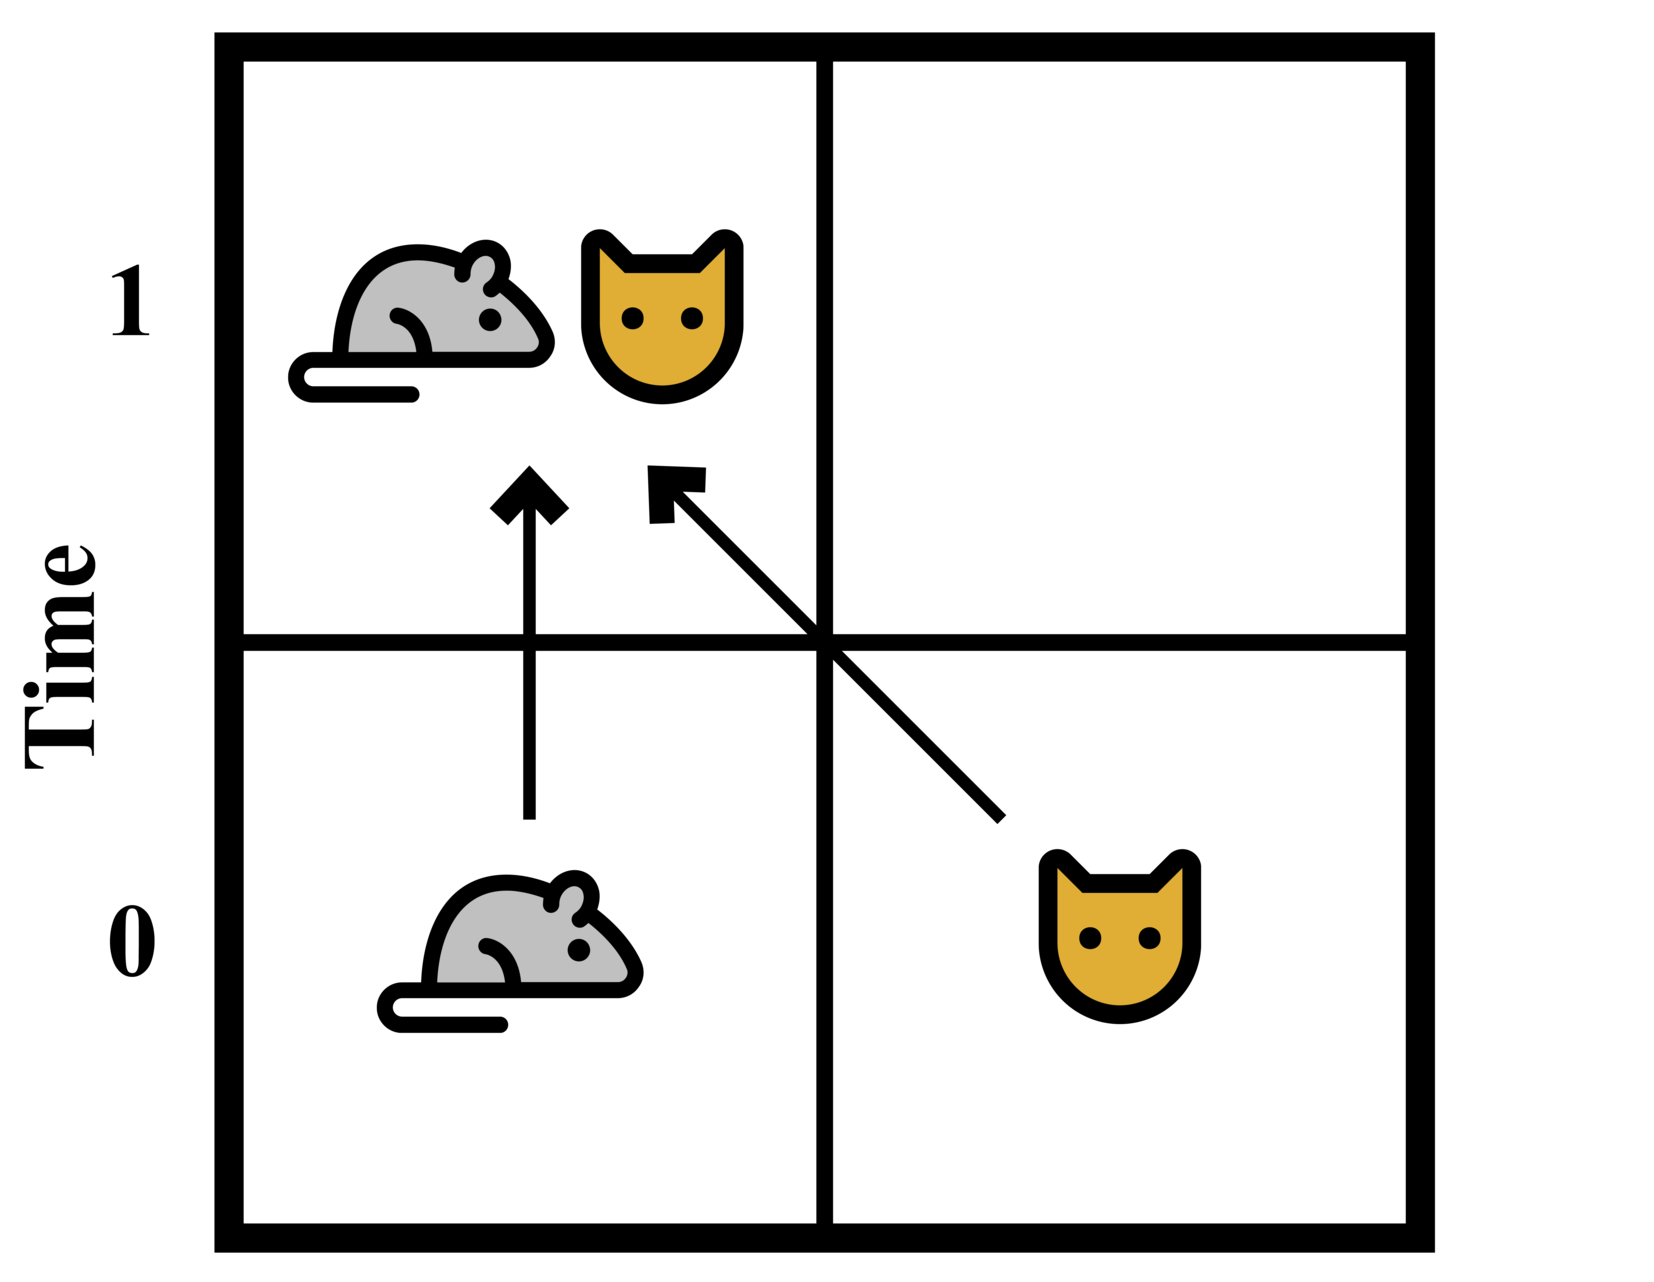
\includegraphics[scale=0.5]{figs/catMouseSm}
	}
	\caption{A simple cat and mouse model.\label{fig:AB-MCMC-1}}
\end{figure}


Let a model timestep consist of a matrix $E$ whose elements $e_{\psi a}$ are the number of agents in state $\psi$ that perform act $a$ in this timestep. For example, the timestep shown in Figure~\ref{fig:AB-MCMC-1} for the cat and mouse example would be
\[
E = \kbordermatrix{
	& A_0 & A_1 \\
	S_0 & 0 & 0 \\
	S_1 & 1 & 0 \\
	S_2 & 0  & 1 \\
	S_3 & 0 & 0 \\
}
\]
where all elements are zero except those representing agent $S_1$ (\textit{right cat}) performing action $A_0$ (\textit{move}) and agent $S_2$ (\textit{left mouse}) performing action $A_1$ (\textit{stay still}).

Let a model trajectory, $T$, be a tensor in $\mathbb{R}^N_{SA}$ that represents $N$ timesteps of a model with $S$ agent states and $A$ actions, so that $T^t_{\psi a}$ denotes the $(\psi, a)^{th}$ element of the $t^{th}$ timestep matrix.

A tensor must satisfy a number of constraints in order to be a valid trajectory of an ABM. Since the elements of a trajectory are counts of agents, they must be non-negative integers. We'll call this the \textit{non-negative integer constraint} and define the set of all non-negative integer tensors
\begin{equation}
\mathcal{I}^N_{SA} = \left\{ T \in \mathbb{R^N_{SA}}: \forall t,\psi, a: T^t_{\psi a} \ge 0, T^t_{\psi a} \in \mathbb{Z}\right\}
\label{nonNegativeInt}
\end{equation}

A trajectory must also be \textit{continuous} by which we mean that the number of agents in each state at the end of timestep $t-1$ must be the number of agents in each state at the beginning of timestep $t$\footnote{This does not mean that agents cannot leave or enter the system, only that if they do then that change must be defined as part of an action.}. We call this the \textit{continuity constraint} and define the set of continuous tensors, with respect to an action function $F$:
\begin{equation}
\mathcal{C}^N_{SA}(F) = \left\{T\in\mathbb{R}^N_{SA}:  \forall \left(  1 \le \bar t < N\right): F^{\psi a}_{\bar\phi} T^{\bar t-1}_{\psi a} = \mathbf{1}^aT^{\bar t}_{\bar\phi a}\right\}
\label{continuous}
\end{equation}
where $F^{\psi a}_\phi$ is the $\phi^{th}$ element of $F(\psi,a)$.


So, the set of valid trajectories, $\mathcal{T}^N_{SA}(F)$, is given by the set of tensors that satisfy \eqref{nonNegativeInt} and \eqref{continuous}.
\begin{equation}
\mathcal{T}^N_{SA}(F) = \mathcal{I}^N_{SA} \cap \mathcal{C}^N_{SA}(F)
\label{SetOfTrajectories}
\end{equation}


\subsection{The posterior}

Given a set of observations, $\Omega$, we'd like to sample from the posterior over the trajectories,
\[
P\left(T \middle| \Omega\right) \propto P(T)P\left(\Omega \middle| T\right)
\]
The prior over the trajectory can be composed from terms involving the agent timestep function, $\pi(\psi,\Psi,a)$, which gives the probability that a single agent will perform action $a$ given that it starts in state $\psi$ and is surrounded by agents $\Psi$. First consider all the agents that are in state $\psi$ at the beginning of timestep $t$. Let $R\in\mathbb{R}_A$ be a vector whose elements $R_a$ are the number of these agents that perform act $a$ in timestep $t$. The probability distribution of $R$ is just a multinomial distribution
\begin{equation}
P\left(R \mid \Psi, \psi\right) = 
\begin{cases}
\Psi_\psi!\prod_a \frac{\pi(\psi,\Psi,a)^{R_ a}}{R_a!} & \text{ if } R_a\mathbf{1}^a = \Psi_\psi \\
0 & \text{otherwise}
\end{cases}
\end{equation}
If we now let $P(\Psi^0)$ be the prior probability over the number of agents in each state at the beginning of the trajectory then the prior over trajectories can be written 
\begin{equation}
P(T) =
\begin{cases}
P(\Psi^0 = T^0_{* c}\mathbf{1}^c)
\prod_{t, \psi}\left(T^t_{\psi b} \mathbf{1}^b \right)!
\prod_a \frac{\pi(\psi, T^{t}_{* d}\mathbf{1}^d,a)^{T^{t}_{\psi a}}}{T^{t}_{\psi a}!} & \text{if } T \in \mathcal{T}^N_{SA}(F) \\
0 & \text{otherwise}\\
\end{cases}
\end{equation}

The likelihood can also be decomposed. Without loss of generality, we take $\Omega$ to consist of some number of observations that are independent of each other given the trajectory, so that $\Omega$ is a set of pairs $(\omega,v)$ that consist of a stochastic observation operator $\omega$ and an observed value $v$ (which may be a vector). We write $P(\omega(T)=v)$ to denote the probability of observation operator $\omega$ making observation $v$ on trajectory $T$. So
\[
P(\Omega|T) = \prod_{(\omega,v) \in \Omega} P(\omega(T)=v)
\]

The posterior can now be written as
\begin{equation}
P(T|\Omega) \propto 
\begin{cases}
\prod_{(\omega,v) \in \Omega,t, \psi, a}
P(\Psi^0 = T^0_{* c}\mathbf{1}^c)
P\left(\omega(T)=v\right)
\left(T^t_{\psi b} \mathbf{1}^b \right)!
\frac{\pi(\psi, T^{t}_{* d}\mathbf{1}^d,a)^{T^{t}_{\psi a}}}{T^{t}_{\psi a}!} & 
 \text{if } T \in \mathcal{T}^N_{SA}(F) \\
0 & \text{otherwise}\\
\end{cases}
\label{posterior}
\end{equation}

The problem we're interested in is how to sample from this distribution. 

In the rest of this paper we'll show how to use the Metropolis-Hastings algorithm to generate samples from equation \eqref{posterior}. The challenge will be to create a proposal function which randomly generates a proposed next sample given the current one. A common strategy with Metropolis-Hastings is to generate a new sample by perturbing one or more elements of the previous sample at random. However, if we do this with a trajectory it's very unlikely that the perturbed tensor will be a trajectory that contains only possible actions and satisfies the observations. So, the proposed next sample would almost certainly be rejected and we'd probably end up stuck on the first sample until we grew old.

\section{Approximating the support of the posterior}
%##########################################

We solve this problem by first approximating the support of the posterior, $\supp(P(T|\Omega))$ (i.e. the set of trajectories that have non-zero probability).

From equation \eqref{posterior}
\begin{equation}
\begin{aligned}
\supp (P( T |\Omega)) = 
& \bigcap_{(\omega,v) \in \Omega,t, \psi, a} \mathcal{T}^N_{SA} \cap \\ 
&\supp(P(\Psi^0 = T^0_{* c}\mathbf{1}^c)) \cap \\
& \supp\left(P\left(\omega(T)=v\right)\right) \cap \\
&\left( \supp\left(\pi(\psi,T^t_{* b}\mathbf{1}^b,a)\right) \cup \left\{T:T^t_{\psi a} = 0\right\} \right)
\end{aligned}
\label{support}
\end{equation}
i.e. in order for $T$ to have non-zero posterior probability, it must be a trajectory of the ABM, it must have a start state that has non-zero prior probability, all the observation likelihoods must be non-zero and each element of $T$ must denote an agent action with non-zero probability.


\subsection{Convex $\mathbb{Z}$-polyhedra and $\mathbb{Z}$-distributions}
%################################################################
\label{BPoly}

Let a $\mathbb{Z}$-polyhedron be a set of tensors whose elements satisfy a set of linear constraints and belong to the set of integers: 
\[
\mathcal{P^N_{SA}} = \left\{ T\in\mathbb{\mathbb{Z}}^N_{SA} : L^{i} \le  C^{\psi ai}_t T^t_{\psi a} \le U^{i} \right\}
\]
$C \in \mathbb{Z}^{SAI}_{N}$, $L \in \mathbb{Z}^I$ and $U \in \mathbb{Z}^I$ for some $I$. This is similar to the $\mathbb{Z}$-polyhedron described in \cite{quinton1996manipulating}).

From equation \ref{SetOfTrajectories} we can see immediately that $\mathcal{T}^N_{SA}$ is a  $\mathbb{Z}$-polyhedron. The supports of the prior, $P(\Psi^0)$, the observations, $P(\omega(T)=v)$, and the agent actions, $\pi(\psi,T^t\mathbf{1},a)$, can often be easily expressed as $\mathbb{Z}$-polyhedra. However, if this is not the case, each of the probability distributions can be expressed as computer programs. Once in this form, it is possible to use a technique known as \textit{abstract interpretation}\cite{cousot1977abstract} using the domain of convex polyhedra\cite{cousot1978automatic}\cite{becchi2018efficient}\cite{fukuda2020polyhedral} to efficiently calculate a convex polyhedron that contains the support (note that it's fine to overestimate the support, i.e. include points that aren't in the support, but not to exclude points that are in the support). Tools to perform abstract interpretation already exist\cite{henry2012pagai}\cite{GN2021} and are used widely in applications such as the verification of safety critical systems\cite{blanchet2003static}. In practice, the generated polyhedra are often reasonably tight approximations of the true support. Calls to a random number generator in the program can be dealt with in the abstract domain by generating a new variable, $r$, that satisfies $0 \le r < 1$ for each call to \texttt{Random()}. These can either be left in as ``auxiliary'' variables in the same way as slack variables, or removed as soon as the variable goes out of scope by finding the convex hull of the projection into a lower dimensional space (by, for example, using the double description method\cite{motzkin1953double}).

If the number of agents is very much smaller than the number of agent states (which is often the case with agent based models) then we may be willing to make the assumption that at any timestep there is at most one agent performing a given action from a given start state (i.e. $\forall \psi, a, t: T^{\psi a}_t \in \{0,1\}$). Under this assumption, which we'll call the \textit{Fermionic assumption}, the set of trajectories is a subset of the corners of the unit hypercube, so the union of any set with the Fermionic trajectories can be expressed as a $\mathbb{Z}$-polyhedron without introducing any approximation.

So, if we let $\mathcal{P}^N_{SA}(f)$ be a $\mathbb{Z}$-polyhedron that over-approximates $\supp(f)$ on the integer points then from equation \eqref{support}
\begin{equation}
\begin{aligned}
\supp(P( T |\Omega)) \subseteq 
& \bigcap_{(\omega,v) \in \Omega,t,\psi, a} \mathcal{T}^N_{SA} \cap \\
& \mathcal{P}^N_{SA}(P(\Psi^0 = T^0_{* c}\mathbf{1}^c)) \cap\\
&    \mathcal{P}^N_{SA}\left(P\left(\omega(T)=v\right)\right) \cap \\
& 
\left(\mathcal{P}^N_{SA}\left(\pi(\psi,T^t_{* b}\mathbf{1}^b,a)\right)
\cup
\left\{T: T^t_{\psi a} = 0\right\}\right)
\\
\end{aligned}
\label{polyhedralSupport}
\end{equation}

The intersection of two $\mathcal{Z}$-polyhedra is easy to construct by just concatenating the constraints
\begin{multline}
\left\{ T\in\mathbb{\mathbb{Z}}^N_{SA} : L \le C^{\psi a*}_{t} T^t_{\psi a} \le U \right\}
\cap \left\{ T\in\mathbb{\mathbb{Z}}^N_{SA} : L' \le D^{\psi a *}_{t} T^t_{\psi a} \le U' \right\} \\
= \left\{ T\in\mathbb{\mathbb{Z}}^N_{SA} : {L \choose L'}  \le  {C^{\psi a*}_t \choose D^{\psi a*}_t} T^t_{\psi a} \le {U \choose U'} \right\}
\end{multline}
so the only difficulty is the union in the final term of \eqref{polyhedralSupport}. To transform this into an intersection we introduce an auxiliary variable $I^t_{\psi a}$ and use the identity
\begin{multline}
\left\{ T\in\mathbb{Z}^N_{SA} : L \le C^{\phi b*}_{s} T^s_{\phi b} \le U \right\}
\cup
\left\{T: T^t_{\psi a} = 0\right\}
=\\
\left\{
T\in\mathbb{Z}^N_{SA}, I^t_{\psi a}\in\{0,1\}:\right.\\
-\infty \le C^{\phi b *}_{s} T^s_{\phi b}
+
(\overline{B}-U)I^{t}_{\psi a}
\le \overline{B},\\
\underline{B} \le C^{\phi b *}_{s} T^s_{\phi b}
+
(\underline{B}-L)I^{t}_{\psi a} \le \infty,\\
0 \le uI^t_{\psi a} - T^t_{\psi a},\\
\left. I^t_{\psi a} - T^t_{\psi a} \le 0
\right\}
\label{implication}
\end{multline}
where $u$ is the maximum value that any element of $T$ can take, the elements of $\overline{B}\in\mathbb{R}^I$ are defined as
\[
\overline{B}^i = \frac{u\sum_{s,\phi,b} \left( C^{\phi bi}_{s} + \left|C^{\phi bi}_{s}\right|\right)}{2}
\]
and the elements of $\underline{B}\in\mathbb{R}^I$ are defined as
\[
\underline{B}^i = \frac{u\sum_{s,\phi,b} \left(C^{\phi bi}_{s} - \left|C^{\phi bi}_{s}\right|\right)}{2}
\]

To see why this identity holds, note first that the constraints on $I^t_{\psi a}$ make it into an indicator variable that is 0 if $T^t_{\psi a}=0$ or 1 otherwise. When $I^t_{\psi a}=1$ the first set of constraints is equal to $C^{\phi b*}_{s} T^s_{\phi b} \le U$ and the second is equal to $L \le C^{\phi b*}_{s} T^s_{\phi b}$ so their intersection is $L \le  C^{\phi b*}_{s} T^s_{\phi b} \le U$ as required, whereas when $I^t_{\psi a}=0$ we have the constraints $\underline{B} \le C^{\phi b*}_{s} T^s_{\phi b} \le \overline{B}$. But $\underline{B}^i$ and $\overline{B}^i$ are lower and upper bounds on the value of $C^{\phi bi}_{s} T^s_{\phi b}$ so this is satisfied for all trajectories, as required.

There are two things worth noting here. Firstly if we make the Fermionic assumption then $I^t_{\psi a} = T^t_{\psi a}$ and the auxiliary indicator variables become unnecessary. Secondly, we must impose a finite value for $u$, the maximum value that elements of the trajectory can take. In practice, this is not a problem as we can give $u$ a value such that the probability of any trajectory of interest having any element larger than $u$ is small.

Using this transformation the support of the posterior can be reduced to a $\mathbb{Z}$-polyhedron

The idea of a $\mathbb{Z}$-polyhedron as the support for a probability distribution naturally leads to the idea of a $\mathbb{Z}$-distribution which is a discrete probability distribution defined over the members of a $\mathbb{Z}$-polyhedron. From the above, it can be seen that the posterior distribution of an ABM trajectory can be expressed as a $\mathbb{Z}$-distribution.

As an illustration, consider a two-timestep trajectory of the cat and mouse model described in section \ref{abmdef}. Suppose we flip a fair coin to decide whether each agent state is occupied or empty at $t=0$. Suppose also that we observe a cat in the left grid-square at time $t=1$. Our aim is to construct a $\mathbb{Z}$-polyhedron, $\mathcal{P}^2_{4\,2}(P(T|\Omega))$, that describes the support of the posterior.

Working through \eqref{polyhedralSupport} term by term, the $\mathcal{T}^2_{4\,2}$ term is just the continuity constraints in \eqref{continuous}, which are already in linear form so we're done. The second term is the support of the prior. This constrains each agent state at $t=0$ to be at most 1, which can be expressed as
\[
\left\{T:T^0_{\psi 0} + T^0_{\psi 1} \le \mathbf{1}_{\psi}\right\}
\]

The third term is the support of the observation. Since we observe a cat in the left grid-square at time $t=1$ we need to add the constraint
\[
T^1_{0 0} + T^1_{0 1} = 1
\]
The final term is the constraint due to agent interactions. The impossible interactions are a mouse staying put when there is a cat on the same gridsquare or moving when there are no cats, which translates to the four cases
\begin{equation}
\begin{aligned}
\supp(\pi(2,T^t_{* a}\mathbf{1}^a,0)) &= \left\{ T: -T^t_{0 0} - T^t_{0 1} \le -1 \right\}\\
\supp(\pi(3,T^t_{* a}\mathbf{1}^a,0)) &= \left\{ T: -T^t_{1 0} - T^t_{1 1} \le -1 \right\}\\
\supp(\pi(2,T^t_{* a}\mathbf{1}^a,1)) &= \left\{ T: T^t_{0 0} + T^t_{0 1} \le 0 \right\}\\
\supp(\pi(3,T^t_{* a}\mathbf{1}^a,1)) &= \left\{ T: T^t_{1 0} + T^t_{1 1} \le 0 \right\}
\end{aligned}
\label{actionConstraints}
\end{equation}
for all t. If, for simplicity, we make the Fermionic assumption by adding the constraints
\[
\mathbf{0}^t_{\psi a} \le T^t_{\psi a} \le \mathbf{1}^t_{\psi a}
\]
then using the identity in \eqref{implication} to take the union of each constraint in \eqref{actionConstraints} with $\left\{T: T^t_{\psi a} = 0\right\}$ finally gives the four constraints
\[
\begin{aligned}
-T^t_{0 0} - T^t_{0 1} + T^t_{2 0} & \le 0\\
-T^t_{1 0} - T^t_{1 1} + T^t_{3 0} & \le 0\\
T^t_{0 0} + T^t_{0 1} + 2T^t_{2 1} & \le 2 \\
T^t_{1 0} + T^t_{1 1} + 2T^t_{3 1} & \le 2
\end{aligned}
\]
for each timestep $t=0$ and $t=1$ to describe the agent interactions.

Taken together, these constraints define a $\mathbb{Z}$-polyhedron that is the set of (Fermionic) trajectories for the cat and mouse ABM, and when combined with equation \eqref{posterior} defines $P(T|\Omega)$ as a $\mathbb{Z}$-distribution.

\section{Sampling from a $\mathbb{Z}$-distribution}
%#################################################

Now that we have shown how to express $P(T|\Omega)$ as a $\mathbb{Z}$-distribution, we now show how to construct a Markov process which will allow us to sample from a $\mathbb{Z}$-distribution.

To do this we need to define
\begin{itemize}
\item a set of Markov states, $\mathcal{M}$

\item a probability measure $P: \mathcal{M} \to \mathbb{R}$ which gives the probability of each Markov state (this need not be normalised, though, as we'll only ever be interested in probability ratios)

\item a stochastic proposal function $f:\mathcal{M} \to \mathcal{M}$ from which we can generate transitions to a new Markov state given the current Markov state

\item a mapping $E:\mathcal{M} \to \mathbb{R}^T_{SA}$ which maps Markov states to trajectories so we can recover the sample.
\end{itemize}

In order to be useable in the Metropolis-Hastings algorithm, the proposal function, $f$, must have the following properties:
\begin{itemize}
	\item For any two Markov states there should exist a set of transitions with non-zero probability which forms a path between those states.
	
	\item For any transition from state $S_a \to S_b$ with non-zero probability, the probability of the reverse transition from $S_b \to S_a$ should also be non-zero. This allows us to attain detailed balance in the Metropolis Hastings algorithm. The average ratio of forward and backward probabilities times the ratio of start and end state probabilities should be close to 1 to ensure that a reasonable proportion of proposals are accepted.
	
	\item Given a current Markov state, there should be computationally efficient ways of generating a proposal and calculating the acceptance probability. 
\end{itemize}


\subsection{The set of Markov states}
%#############################################

Given a $\mathbb{Z}$-polyhedron, we split the constraints into two sets: equalities (i.e. those whose lower and upper bound have the same value) and inequalities (i.e. those whose lower and upper bounds differ):
\begin{equation}
\mathcal{P} = \left\{T \in \mathbb{Z}^N_{SA}: L^i \le C^{\psi ai}_t T^t_{\psi a} \le U^i \cap D^{\psi ai}_t T^t_{\psi a} = E^i \right\}
\label{zPolySupport}
\end{equation}

Suppose there are $N_e$ equality constraints (i.e. $E$ is an $N_e$ dimensional vector of integers) and we partition the elements of $T$ into `basic' and `non-basic' elements, so that there are exactly $N_e$ basic elements and $N\times S \times A - N_e$ non-basic elements.

A partition of $T$ can be defined as a pair of tensors $Q\in\{0,1\}_{SAN_e}^{N}$ and $R\in\{0,1\}_{SAJ}^{N}$, where $J=NSA - N_e$. $Q$ and $R$ take vectors of basic, $X\in\mathbb{R}^{N_e}$, and non-basic, $Y\in\mathbb{R}^J$, variables and pack them into a trajectory tensor, without changing their values. More formally, $Q$ and $R$ should satisfy
 \[
Q_{\psi ai}^{t} \mathbf{1}^i + R_{ \psi  aj}^{t} \mathbf{1}^j =  \mathbf{1}^t_{\psi a}
 \]
 \[
Q_{\psi ai}^{t} \mathbf{1}_t^{\psi a} = \mathbf{1}_i
 \]
 \[
R_{\psi aj}^{t} \mathbf{1}_t^{\psi a} = \mathbf{1}_j
\]
Given the partition, we can map from vectors to tensors
\begin{equation}
T^{t}_{\psi a} =  Q_{\psi ai}^{t} X^i + R_{ \psi  aj}^{t} Y^j
\label{trajXY}
\end{equation}
If we now let
\begin{equation}
B_i^k = D^{\psi ak}_{t}Q_{\psi a i}^{t}
\label{Bmatrix}
\end{equation}
and
\[
N_j^k = D^{\psi ak}_{t}R_{\psi aj}^{t}
\]
then we can write the equality constraints as
\begin{equation}
B_i^kX^i + N_j^kY^j = E^k
\label{eqconstraints}
\end{equation}

Now, since there are $N_e$ basic variables and $N_e$ equality constraints, $B$ is square so if we choose the basic variables in such a way as to ensure that $B$ has an inverse then
\begin{equation}
X^i = (B^{-1})^i_k(E^k + N_j^kY^j)
\label{basicvars}
\end{equation}
inserting this into \eqref{trajXY} gives
\begin{equation}
T^t_{\psi a} =  Q_{\psi ai}^{t}(B^{-1})^i_k(E^k + N_j^kY^j) + R_{\psi aj}^{t } Y^j
\label{markovtotrajectorytensor}
\end{equation}
or equivalently
\begin{equation}
T^t_{\psi a} =  K^t_{\psi a} + M^{t}_{\psi aj} Y^j
\label{markovtotrajectory}
\end{equation}
where
\[
K^t_{\psi a} = Q_{\psi ai}^{t} (B^{-1})^i_kE^k
\]
and
\[
M^{t}_{\psi aj} = Q_{\psi ai}^{t} (B^{-1})^i_kN_j^k + R_{\psi aj}^{t}
\]
If we also choose the basic variables such that all elements of $B^{-1}$ are integer then we can define the set of Markov states to be
\[
\mathcal{M} = \left\{ Y \in \mathbb{Z}^J: \forall i:0 \le Y_i \le u \right\}
\]
where $u$ is the upper limit on the occupancy of agent actions, and map each Markov state, $Y$, to a unique integer trajectory using \eqref{markovtotrajectory}.

\subsection{The probability of a Markov state}

Given a Markov state, $Y$, that satisfies $0 \le Y_j \le u$, the associated trajectory given by equation \eqref{markovtotrajectory} is guaranteed to satisfy all the equality constraints. However, there is no guarantee that the basic variables given by eq \eqref{basicvars} will be within their bounds or that the inequality constraints will be satisfied. To deal with this we introduce the concept of \textit{infeasibility} which is a measure of how far a Markov state is from being feasible.

Given the inequality constraints of the $\mathbb{Z}$-distribution (including the upper and lower limits of the trajectory elements themselves)
\[
L^i \le C^{\psi ai}_{t} T^t_{\psi a} \le U^i
\]
using \eqref{markovtotrajectory} this can be written as
\begin{equation}
L^i \le J^i + Q_j^i Y^j \le U^i
\label{ineqconstraints}
\end{equation}
where
\[
J^i = C^{\psi ai}_{t} K^t_{\psi a}
\]
and
\[
Q_j^i = C^{\psi ai}_{t}M^{t}_{\psi aj}
\]

let the infeasibility of the $i^{th}$ constraint, $\iota(Y)_i$, be defined to be equal to 0 if the constraint is satisfied or equal to the distance to the nearest bound otherwise
\[
\iota(Y)_i =
\begin{cases}
L^i- J^i - Q_j^iY^j & \text{if }J^i + Q_j^iY^j<L^i\\
J^i + Q_j^iY^j-U^i & \text{if }J^i + Q_j^iY^j>U^i\\
0 & \text{otherwise}
\end{cases}
\]
and let the total infeasibility be the sum of infeasibilities of all constraints
\[
\iota(Y) = \sum_i \iota(Y)_i
\]
So, each Markov state is associated with a total infeasibility with respect to the inequalities of the $\mathbb{Z}$-distribution. 

If the infeasibility is zero, then all the constraints are satisfied and the probability is defined by the $\mathbb{Z}$-distribution
\[
P(Y) = P(K^t_{\psi a} + M^{t}_{\psi aj}Y^j)
\]

If the infeasibility is not zero, then the probability is defined in the following way. Given an upper bound on the trajectory's elements, $u$, we define the \textit{clamped} trajectory
\[
\overline{\underline{T^t_{\psi a}}} = 
\begin{cases}
0 & T^t_{\psi a}<0\\
u & T^t_{\psi a}>u\\
T^t_{\psi a} & \text{otherwise}
\end{cases}
\]

Furthermore, let $H_t^{\psi a}$ be a log-linear approximation to the target $\mathbb{Z}$-distribution so that for feasible trajectories
\[
H_t^{\psi a}T^t_{\psi a} \approx \log(P(T))
\]
For infeasible trajectories, we define the probability, $P_\iota$, as
\begin{equation}
\log(P_\iota(Y)) = \sum_{t \psi a} H_t^{\psi a}\overline{\underline{K^t_{\psi a}+M^{t}_{\psi aj}Y^j}} + \kappa\iota(Y)
\label{loglinprob}
\end{equation}
where $\kappa < 0$ is a tunable parameter.

The probability of a Markov state, $Y$, is now given by
\begin{equation}
P(Y) =
\begin{cases}
P(Y) & \text{if } \iota(Y) = 0\\
P_\iota(Y) & \text{if } \iota(Y) > 0\\
\end{cases}
\end{equation}

This means that infeasible states have non-zero probability, so the Markov chain will pass through some infeasible states.  However, if we just ignore these and only take samples from feasible states then we end up with samples of the target $\mathbb{Z}$-distribution. Allowing the Markov chain to pass through infeasible states has the advantage of ensuring that there exists a path between any two feasible states and improves mixing. The disadvantage is the computational cost of moving through infeasible states that don't generate useful samples.

The infeasible Markov states are distributed as a Boltzmann distribution with a ``temperature'' of $\frac{-1}{\kappa}$.  It has been shown that thermodynamic systems of this type are able to solve large integer optimisation problems \cite{kirkpatrick1983optimization}. In our case, we don't need to change the temperature during the sampling process, but we do need to choose a value for $\kappa$. Higher temperatures will increase mixing in the Markov chain, but will also increase the proportion of time spent in infeasible states so we need to find a temperature that is high enough to ensure good mixing of the chain but low enough to ensure a reasonable proportion of samples are feasible. We have found that a good rule of thumb is to set the temperature so that 50\% of the states in a chain are infeasible.

\subsection{Transitions between Markov states}

Given a Markov state, we can transition to another state by choosing an element of  $Y$ and perturbing it by $\pm 1$ (or, if the element is on one of its bounds then to perturb it away from the bound in the feasible direction. In the case of Fermionic trajectories, the elements of $Y$ are always on their bounds so there is always exactly one perturbation per element: a swap to the other bound). This defines the set of transitions between Markov states. Let the set of all Markov states reachable from state $Y$ be denoted by $\mathcal{D}(Y)$. 

\subsubsection{The probability of transitions}

The probability of a transitions from $Y$ to $Y'$ is defined to be
\[
P(Y \to Y') = \frac{\min\left(1, \frac{P_\iota(Y')}{P_\iota(Y)}\right)}{S(Y)} 
\]
where $P_\iota$ is the log-linear probability defined in \eqref{loglinprob} and
\[
S(Y) = \sum_{Y'\in \mathcal{D}(Y)}\min\left(1, \frac{P_\iota(Y')}{P_\iota(Y)}\right)
\]
Note that this is irrespective of whether $Y$ or $Y'$ are feasible.

Given this, the Metropolis-Hastings acceptance probability is
\[
\alpha = \frac{P(T')P(Y' \to Y)}{P(T)P(Y \to Y')} = 
\frac{P_\iota(Y)}{P(Y)} \frac{P(Y')}{P_\iota(Y')}  \frac{S(Y)}{S(Y')}
\]

When $Y$ is infeasible $\frac{P_\iota(Y)}{P(Y)} = 1$. When $Y$ is feasible $P_\iota(Y)$ approximates $P(Y)$ so their ratio should be close to 1. Finally, $S(Y)$ will not change very much between transitions so the ratio $ \frac{S(Y)}{S(Y')}$ should also be close to 1 meaning that the acceptance probability should also be close to 1.

\subsection{Choosing a basis}

The definition of the Markov chain depends on a partition of the trajectory into basic and non-basic variables such that $B$ in equation \eqref{Bmatrix} has an integer inverse $B^{-1} \in \mathbb{Z}^{N_e}_{N_e}$. In general there exist many possible partitions so it remains to define a method of choosing one. The choice we make affects the way Markov states are mapped to trajectories via equation \eqref{markovtotrajectory} and how infeasibility is calculated via equation \eqref{ineqconstraints}, where the columns of $Q$ can be thought of as basis vectors in a \textit{constraint space} and $Y$ as a coordinate on the grid formed by that basis. The Markov chain can be seen as a random walk around this grid. If we choose a basis that consists of very dense basis vectors then the Markov states adjacent to a feasible trajectory are likely to have high infeasibility and low probability, leading to slow mixing of the chain, so we aim to choose a basis that has sparse basis vectors in the constraint space. This has the additional advantage that when we transition between adjacent Markov states, the probability distribution over transitions changes in only a few dimensions. This means we can use a binary tree to efficiently update and draw from the probability distribution over transitions\cite{TangMutableCategorical}.

Starting with a $\mathbb{Z}$-polyhedron expressed in the form
\[
\mathcal{P} = \left\{T \in \mathbb{Z}^N_{SA}: L^i \le C^{\psi ai}_t T^t_{\psi a} \le U^i \cap D^{\psi ai}_t T^t_{\psi a} = E^i \right\}
\]
suppose we begin with no basic variables so that $R$ is an arbitrary ordering of the elements of a trajectory
\[
T^t_{\psi a} = R^t_{\psi a j}Y^j
\]
If we let
\[
W^*_j = {D^{\psi a*}_t R^t_{\psi aj} \choose C^{\psi a*}_t R^t_{\psi aj}}
\]
and
\[
F = {E \choose \mathbf{0}}
\]
then
\begin{equation}
\mathcal{P} = \left\{T \in \mathbb{Z}^N_{SA}: {\mathbf{0} \choose L} \le W Y - F \le {\mathbf{0} \choose U} \right\}
\label{jointconstraints}
\end{equation}

We use a greedy algorithm to eliminate variables from $Y$ and equality constraints from $W$ one at a time until $N_e$ variables and all equality constraints have been eliminated. The remaining variables in $Y$ will make up the non-basic variables and the remaining constraints will define a basis in the constraint space.

Given a set of constraints in the form \eqref{jointconstraints}, if we choose an element $W^i_j$ to be a \textit{pivot point} such that $W^i_j = \pm1$ and $i < N_e$, we can eliminate variable $Y^j$ and the equality constraint $W^*_i$ by performing Gaussian elimination on the $j^{th}$ column of $W$ and removing row $i$ and column $j$ from $W$, so that
\[
{\mathbf{0} \choose L} \le GWH\hat{Y} - GF \le {\mathbf{0} \choose U}
\]
where $G\in \mathbb{Z}^{N_e-1}_{N_e}$
\[
G =  
\begin{pmatrix}
1 &  & &-\frac{W^0_j}{W^i_j} & & &\\
& \ddots & &\vdots & & &\\
& & 1 & -\frac{W^{i-1}_j}{W^i_j} & & &\\
& &  & -\frac{W^{i+1}_j}{W^i_j} & 1 & &\\
& & & \vdots & & \ddots &\\
& & & -\frac{W^n_j}{W^i_j} & & &1\\
\end{pmatrix}
\]
$\hat{Y}$ is $Y$ with the $j^{th}$ element removed and $H$ is the identity matrix with the $j^{th}$ column removed. Letting $\hat{W} = GWH$ and $\hat{F} = GF$ recovers the canonical form
\[
{\mathbf{0} \choose L} \le \hat{W}\hat{Y} - \hat{F} \le {\mathbf{0} \choose U}
\]

Since $W^i_j = \pm1$, $B^{-1}$ exists and is integer, so $\hat{Y}$ maps to a unique integer trajectory, as required.

Note that $WG$ differs from $G$ in $(\left|G^*_j\right|_0-1)(\left|G^i_*\right|_0-1)$ elements, where $\left|\cdot\right|_0$ is the number of non-zero elements in a tensor. So, this gives an upper bound on the increase in L0-norm, $\left|WG\right|_0 - \left|G\right|_0$ and so gives a measure of how much sparsity may be lost by pivoting on $W^i_j$.  It has been found that choosing $W^i_j$ to be the element that minimises this measure (known as the Markowitz criterion) is a computationally efficient way of maintaining the sparsity of a matrix while performing Gaussian eliminatination\cite{markowitz1957elimination}\cite{maros2002computational}\cite{suhl1990computing}. So, in order to find a sparse basis we choose the element that minimises $(\left|G^*_j\right|_0-1)(\left|G^i_*\right|_0-1)$, perform the elimination and repeat until no more equality constraints remain, $N_e=0$.

\section{Spatial predator-prey demonstration}

We demonstrate the above techniques on a 32x32 grid of ``predator'' and ``prey'' agents. At each timestep a prey agent either moves to an adjacent grid-square (i.e. up, down, left or right with equal probability), dies or gives birth to another prey agent on the an adjacent grid-square. Predators also either move to an adjacent grid-square, die or give birth. However, predators only give birth when there is at least one prey on an adjacent grid-square. In addition, if a prey has any predators on adjacent grid-squares there is a chance it may be eaten. The probability of each behaviour is shown in table \ref{rates}.

\begin{table}
	\begin{center}
		\begin{tabular}{llllc}
		\hline
		Aget type & Adjacent agents & Behaviour & Probability\\
		\hline
		Prey & No predators & die &        0.100\\
			& & give birth &        0.156\\
			& & move &        0.744\\
			& &&\\
		Prey & Predators > 0 & die &        0.100\\
			& & give birth &        0.156\\
			& & be eaten &        0.300\\
			& & move &        0.444\\
			& &&\\
		Predator  & No prey & die  &      0.100\\
			& & move &        0.900\\
			& &&\\
		Predator  & Prey > 0 & die  &      0.100\\
			& & give birth &        0.300\\
			& & move &        0.600\\
		\hline& 
		\end{tabular}
	\end{center}
	\caption{The probabilities of each behaviour in the predator-prey model}
	\label{rates}
\end{table}

\begin{figure}
	\centering
	\resizebox{0.5\textwidth}{!}{
		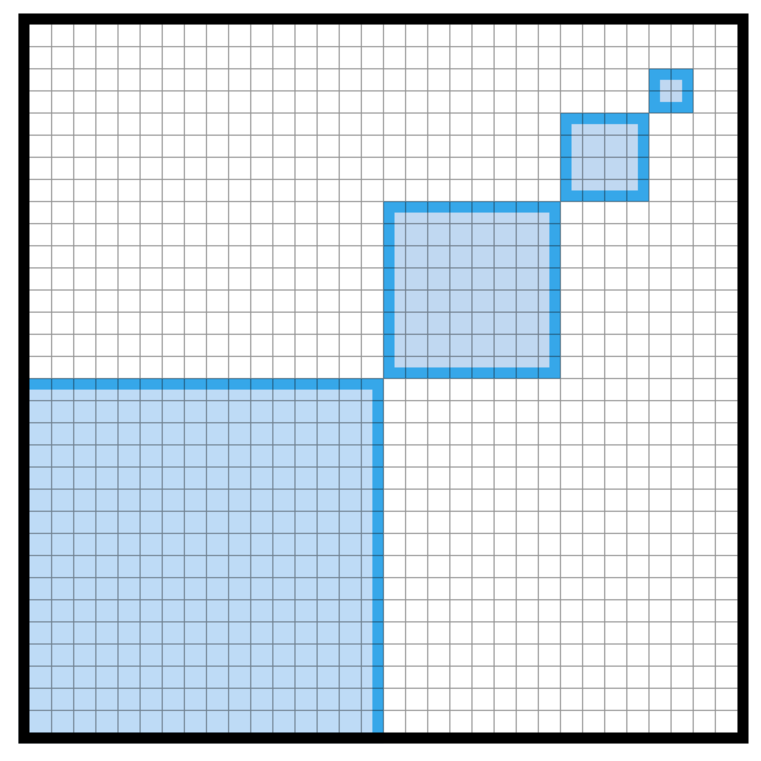
\includegraphics[scale=0.5]{figs/gridRegionsSm.png}
	}
	\caption{Summary statistics consist of the total number of agents in each of the four shaded regions.}
	\label{figRegions}
\end{figure}

\begin{figure}
	\centering
	\resizebox{0.8\textwidth}{!}{
		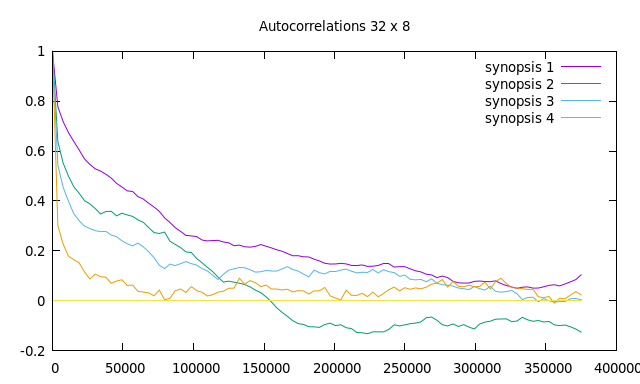
\includegraphics{figs/autocorrelation.png}
	}
	\caption{Mean autocorrelation for each scalar of the summary statistics, averaged over all chains.}
	\label{figAutocorrelation}
\end{figure}

\begin{figure}
	\centering
	\resizebox{0.8\textwidth}{!}{
		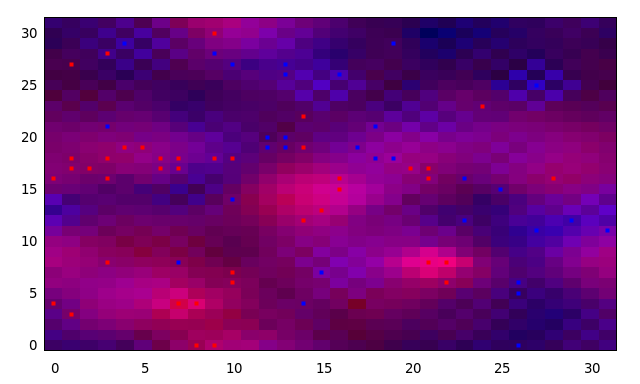
\includegraphics{figs/endState.png}
	}
	\caption{Mean number of agents in each gridsquare after the last timestep, averaged over all samples. Blue represents predator, red represents prey. The dots represent the final positions of agents in the simulation from which the observations were generated. The background colour of each square has red/blue intensity proportional to the log of the mean number of prey/predators in that square, respectively.}
	\label{figEndState}
\end{figure}


Simulated observation data was generated by profroming a forward simulation of the model. The number of predators and prey in each gridsquare at the start of the simulation was drawn from a Poisson distribution with rate parameter $\lambda = 0.05$. The model was then simulated forward for 16 timesteps. At each timestep, each gridsquare was observed with a probability of 0.02. If an observation was made, the number of predators in the gridsquare was observed. In order to simulate observational noise, each predator was observed with probability 0.9 (i.e. the number observed was drawn from a Binomial distribution). The same procedure was then repeated for prey.

Four separate Markov chains of 1,500,000 samples each were generated from the posterior using the method described above. The start state for each chain was drawn from the prior (i.e. model trajectory without any observations). The first 200,000 samples of each chain were discarded and the remaining samples were split into first and last halves to give 8 sample sequences in total. 

In order to assess the convergence of the chains, a set of summary statistics were calculated for each sample of each chain. The summary statistics consisted of the total number of agents within the shaded regions shown in figure \ref{figRegions} measured after the last timestep of the trajectory. This arrangement of regions was chosen in order to capture the convergence at different spatial scales. From the summary statistics, we calculated the the Gelman-Rubin diagnostic \cite{gelman1992inference}, and approximated the autocorrelation at various time lags. Using the notation $x_{ij}$ to refer to a scalar statistic of the $i^{th}$ sample of the $j^{th}$ sequence, given $m$ sequences of $n$ samples each, let $\bar{x}_j$ be the mean of the $j^{th}$ sequence and $\bar{x}$ be the mean over all sequences
\[
\bar{x}_j = \frac{1}{n}\sum_{i=1}^n x_{ij}, \bar{x} = \frac{1}{m}\sum_{j=1}^m \bar{x}_j
\]
let $W$ be the within-sequence variance
\[
W = \frac{1}{m} \sum_{j=1}^m \frac{1}{n-1} \sum_{i=1}^n (x_{ij} - \bar{x}_j)^2
\]
and $B$ be the between-sequence variance
\[
B = \frac{n}{m-1}\sum_{j=1}^m (\bar{x}_j - \bar{x})^2
\]
Following\cite{gelman2013bayesian}, an overapproximation of the true variance of the statistic can be calculated as
\[
\widehat{\text{var}}^+ = \frac{n-1}{n}W + \frac{1}{n}B
\]
and the Gelman-Rubin statistic can be defined as
\[
\hat{R} = \sqrt{\frac{\widehat{\text{var}}^+}{W}}
\]
This gives a measure of the uncertainty in the standard deviation of the statistic due to the fact that we have only taken a finite number of samples. If this number is close to 1, then we have some justification in believing that we have taken enough samples.

Also following\cite{gelman2013bayesian}, we approximated the autocorrelation as
\[
\hat{\rho}_t = 1 - \frac{V_t}{2\widehat{\text{var}}^+}
\]
where
\[
V_t = \frac{1}{n-t} \sum_{i=1}^{n-t} (x_i - x_{i+t})^2
\]

Figure \ref{figAutocorrelation} shows $\hat{\rho}_t$ as a function of $t$ for each scalar in the summary statistics. A decline of $\hat{\rho}_t$ to zero long before $t$ reaches the total number of samples, shows good convergence of the chain. The rate of this decline can be used to calculate the effective number of samples, defined as
\[
\hat{n}_e = \frac{mn}{1 + 2\sum_{t} \hat{\rho}_t}
\]
where the sum runs until $\hat{\rho}_t \le 0$. This approximates of the number of samples from a perfect IID sampler that would give the same uncertainty in the mean of the statistic.

Finally, figure \ref{figEndState} shows the mean number of agents at the end of the simulation, averaged over all samples. This is a visual way of showing that the observations have given rise to a posterior that gives some information about the true positions of the agents.
 

\section{Limitations and further work}

[column generation for larger internal state]

[automatic linearisation]

[extension to PPL]

[model error]

\section{Conclusion}

We have described and demonstrated an algorithm to sample model trajectories from the posterior distribution of an agent based model given a set of observations. This allows us to use ABMs to perform inference about unobserved variables given a set of observations and to make forecasts given observations up to the present.

As presented, the algorithm is not applicable to agents that have a large amount of internal state (above a few bytes) but we suggest ways that this algorithm can be extended to apply in these cases.

Data assimilation with agent based models is currently in its infancy, and more powerful techniques for performing Bayesian inference with ABM could transform the usefulness and applicability of these models. The 

%\bibliographystyle{unsrtnat}
%\bibliographystyle{apalike} 
\bibliographystyle{apacite}
\bibliography{references}

\end{document}
